%%%%%%%%%%%%%%%%%%%%%%%%%%%%%%%%%%%%%%%%%%%%%%%%%%%%%%%%%%%%%%%%%%%%%%%%%%%%%%%%
% Template for USENIX papers.
%
%%%%%%%%%%%%%%%%%%%%%%%%%%%%%%%%%%%%%%%%%%%%%%%%%%%%%%%%%%%%%%%%%%%%%%%%%%%%%%%%
\documentclass[letterpaper,twocolumn,10pt]{article}
\usepackage{usenix}

% to be able to draw some self-contained figs
\usepackage{tikz}
\usepackage{amsmath}
\usepackage{xxxnotes}

% inlined bib file
\usepackage{filecontents}

%-------------------------------------------------------------------------------
\begin{filecontents}{\jobname.bib}
%-------------------------------------------------------------------------------
@incollection{positiongdpr,
  title={Position: Gdpr compliance by construction},
  author={Schwarzkopf, Malte and Kohler, Eddie and Kaashoek, M Frans and Morris, Robert},
  booktitle={Heterogeneous Data Management, Polystores, and Analytics for Healthcare},
  pages={39--53},
  year={2019},
  publisher={Springer}
}
\end{filecontents}

%-------------------------------------------------------------------------------
\begin{document}
%-------------------------------------------------------------------------------

%don't want date printed
\date{}

% make title bold and 14 pt font (Latex default is non-bold, 16 pt)
\title{\Large \bf 6.824 Project Proposal: Designing GDPR Compliant-by-Construction Systems}

%for single author (just remove % characters)
\author{
{\rm Lillian Tsai}\\
MIT
% copy the following lines to add more authors
% \and
% {\rm Name}\\
%Name Institution
} % end author

\maketitle

%Flesh out the exact problem you will be addressing and how you will go about solving it. By the proposal deadline, you must submit a proposal (less than a page) describing: your group members list, the problem you want to address, how you plan to address it, and what are you proposing to specifically design and implement. Submit your proposal to https://6824.scripts.mit.edu/2020/handin.py/. We'll tell you whether we approve, or not, and give you feedback.

%-------------------------------------------------------------------------------
\section{Problem Statement}
%-------------------------------------------------------------------------------
Websites such as Facebook, Twitter, and Google have historically controlled the storage and processing of their users' data.
A user uploading data to such services would forfeit the right to control that data, allowing the website to dispense and retain her data, perhaps indefinitely.
With the recent introduction of the European Union's General Data Protection Regulation (GDPR) laws, 
users gain explicit rights to own their data: they have the right to obtain, as well as completely erase, any of their data stored by the service. However, implementing GDPR-compliant services is not straightforward, as current system designs were not designed with user data ownership as a first principle.

In this project, I will design and prototype a new data storage model loosely based upon the one proposed by Schwarzkopf et al.~\cite{positiongdpr}, which suggests new abstractions for GDPR compliant-by-construction systems. In this model, each end-user of a web service maintains their own mini-database (a ``user shard'') that holds all information pertaining to them and related to this service. The data available to the shared service is the cumulative sum of all the underlying user shards, which the
service can combine and process. Each user grants the service a timed lease to the data in their shard, permitting the service to store and compute over this data for a limited time. The service promises to remove the provided data and any derived computation on lease expiration.
This model of data storage raises many questions that this project aims to investigate:
\begin{itemize}
    \item What is the impact of logically (or physically) disjoint user data? How will the movement of data from user-owned shards to shared storage affect service load and throughput?
    \item What does it mean to "own" data in the context of a specific web application? For example, who owns a private messaging conversation on Facebook, or a reply made on Twitter?
\end{itemize}

%-------------------------------------------------------------------------------
\section{Design Sketch}
%-------------------------------------------------------------------------------
The system model proposed will consist of two components: 
(1) end-user clients, each with a user shard (mini-database) that contains
that specific user's data; 
(2) a shared service with access to the cumulative sum of all user shards, with the ability to combine and process this data.
Users subscribe to and update the service via RPC calls (see Section~\ref{sec:rpcs}).
Figure~\ref{fig:design} shows the flow of data through the system.

\begin{figure}
    \centering
    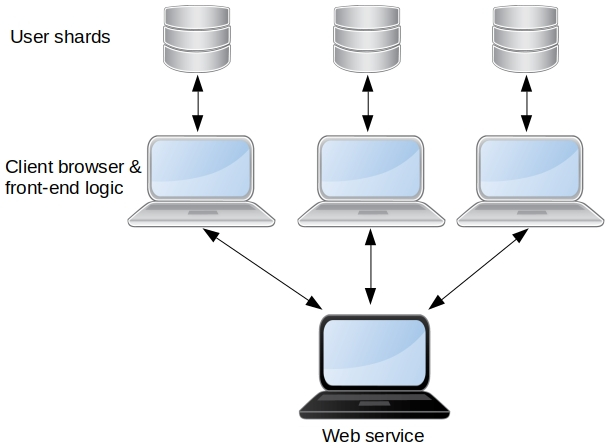
\includegraphics[width=0.4\textwidth]{usershards}
    \caption{Clients privately store and update data in user shards, and send updates to a shared web service. Clients can then read (potentially processed) data from the web service.}
    \label{fig:design}
\end{figure}

A client must be aware of the objects manipulated by the service (e.g., posts, comments, photos, etc.) in order
to correctly send shard data updates to the service.
A user shard would be inaccessible by the service or other users; this could be either locally
on the client itself or in a Cloud storage system such as AWS, 
depending on the privacy requirements of the user, the amount of user data, and
the cost the user (or service) is willing to pay.

While data flows explicitly between client and service via RPC calls, 
the service can only retain data for a limited time, after which the user's
data will be implicitly and automatically revoked from the service (and any derived 
data).
This is supported via \emph{leases}, which are described in
more detail in Section~\ref{sec:leases}. 
We note that automatic revocation goes beyond
the requirements of the GDPR; our system design includes leases in order to  
strengthen the notion of user data ownership.

\subsection{RPC Interface}
\label{sec:rpcs}
RPCs between client and service fall into three classes of operations:
\begin{enumerate}
    \item shard management operations
    \item write operations (including insertions, modifications, and deletions)
    \item read operations
\end{enumerate}

User shard management operations include operations such as \texttt{subscribe} and \texttt{unsubscribe}. 
A \texttt{subscribe} operation establishes a connection with the service if one does not exist, and contains all data and writes that the service has not received from the client. This may include writes that were logged but not yet sent to the service (see Section~\ref{sec:logging}) due to a crash, or data that had been revoked due to a lease expiration (see Section~\ref{sec:leases}) or \texttt{unsubscribe} operation (\texttt{unsubscribe} removes all user data from the service).

The client refuses any updates that occur while unsubscribed: this ensures that writes appear consistently to every user, i.e., 
users only receive successful responses when the change has been reflected by the service and is visible to others.
This prevents, for example, a situation in which a user issues a (successful) delete-post request while its client is unsubscribed, but another subscribed client adds comments onto the not-yet-removed post.

Write and read operations are implemented in an application-specific manner.
For example, a social network service may include write operations to create new posts,
delete posts, make comments, or edit post text.

\subsection{Consistency Model}
\label{sec:logging}
For every write, the client first applies the write to the user shard, then 
sends an RPC to the service and waits for a successful reply.
An alternative approach would be to first send the RPC to the service, and then only apply the write to the user shard. 
We choose the former approach because it more naturally reflects the invariant that the shared service is the 
cumulative sum of all user shards.

With either approach, the service's application order determines the linearization point of the operation.
For example, if one client deletes a post, and another client concurrently comments on the post,
the service can either apply the deletion first and return \texttt{error} to the commentor, or post the comment first
and return \texttt{success}.

In order to ensure that writes provide a consistent view to all users even in the face of disconnects or crashes 
while RPCs are in flight, we imagine that the client will need to implement a persistent write-ahead-log (WAL). 
Prior to applying the write to its database and sending the service an RPC, the client logs the write information; 
the log entry is marked committed (so the log may later be truncated) when the client write receives a successful RPC reply. 
During recovery from failure or upon subsequent \texttt{subscribe}s, the client issues any uncommitted writes remaining in the log. Both service and client-side code must ensure that these writes are either idempotent, or detect duplicate requests via 
monotonically increasing identifiers for every write (not applying any write with a identifier lower than that of the last applied write).

In order to improve performance, we predict that we will have to perform writes in batches (so every batch, rather than every write, would require two disk writes). To allow for reads to proceed even when writes are batched, 
this may require weakening the consistency model such that reads can observe state prior to any write that has returned but been batched. Or perhaps there can be client-side read-my-writes resolution; however, the client may not necessarily have enough information to know how these writes would be processed by the service.
%\XXX{I actually don't see any read-my-writes issues here---the client won't be able to proceed with a subsequent read until 
%a write has been both processed by the service and the user shard. 
%If we were to implement batching, it seems like any client read would require that all batched writes be issued and acknowledged by the service before the read returns, because the client wouldn't necessarily have enough information to know how the service
%would process all writes. Am I forgetting something trivial here?}

\subsection{Leases}
\label{sec:leases}
In order to allow for automatic data revocation after some defined timeout, 
a user's data is associated with a \emph{lease}.
While a lease is still valid, the service may process and share a user's data
unless it is explicitly withdrawn. Lease renewals occur when a user contacts the
service: users may send heartbeats (empty update RPCs), a normal update, a read request,
or simply resubscribe to the service.
For simplicity, our first prototype design requires mandatory, coarse-grained leases: every user RPC 
must specify a lease expiration time, and the lease applies to all of the user's data.

We can also imagine an alternative design, in which every piece of user data has a separate lease, or
where user data by default has a set lease time. However, this complicates the system design, as either (or both)
the user and the service must track individual leases for potentially hundreds or thousands of distinct pieces
of data. However, given particular service applications, this lease design may be inevitable: for example, users may wish to 
lease their post data for a shorter period of time than their likes on posts.

Given this lease design, the service must ensure that it removes all user data 
from any of its local when the lease time is up.
If the user issues any RPCs after the lease has expired, 
the service will need to re-request all user data,
and will notify the user by returning an error code.
The user will then issue a \texttt{subscribe} request with the required data.

\subsection{Inter-user Dependencies and Revoked Data}
Because user data can be semantically dependent upon another user's (like a comment on a post, or private
messages between two users),
revoking one user's data can raise thorny questions about how to handle other related data
written by other users.
For example, what will happen if a comment is made on a post that another user deletes? Should the comment be removed? Or does this comment belong to the user who posted it? 

In our initial design, whatever a user writes is said to be owned by the user; if the 
data depends on a piece of data revoked by another user (e.g., a comment on a revoked post),
the shared service could enforce that the comment is now orphaned beneath an anonymous post
unrelateable to the original user, or that the comment be inaccessible.
This is similar to the idea of referential integrity: when the user revokes 
a piece of data, any references to that data in the service no longer has any meaning.

Note that this means that upon a resubscribe, a user's data may end up in a different ``place'' 
in the service than prior to revocation, depending on the actions of other users.
For example, revoking a user's post may orphan all post comments made by others,
and a resubscribe of that user may no longer be able to associate the post with 
its comments. 
This stance ensures that a user cannot be remembered even via a 
``deleted'' placeholder, at the cost of losing some information associating one 
user's data with another's when that user's data is revoked.

%-------------------------------------------------------------------------------
\section{Implementation Details}
%-------------------------------------------------------------------------------
The system prototype will be written in Go. Each user shard will be represented as a MySQL database, and the service's materialized views as an in-memory hashtable (coupled with in-memory copies of each user shard). Each client owning a user shard communicates via Go RPCs with the service, which initially will be non-fault-tolerant (a single replica).

The initial system will be a simple model of a service that offers the ability to post articles and either up or downvote others' articles (similar to the Lobsters community).
Users have the ability to update or create new articles, as well as update or create their votes.
The database schema for user shards is as follows:
\begin{itemize}
    \item Articles Table:
        \begin{itemize}
            \item article ID (unique)
            \item content (typically a url)
            \item timestamp (last edited)
        \end{itemize}
    \item Votes Table:
        \begin{itemize}
            \item timestamp (last edited)
            \item article ID (unique)
            \item isUpvote
        \end{itemize}
\end{itemize}

\noindent
The service stores materialized views for the following queries:
\begin{verbatim}
 createViewVoteCountQ = 
    CREATE VIEW VoteCount as 
    SELECT Vote.aid, COUNT(DISTINCT uid) 
    AS votes 
    FROM Vote GROUP BY Vote.aid;

 articleWithVoteCountQ = 
    SELECT Article.aid, title, content, 
           VoteCount.votes 
    AS votes 
    FROM Article, VoteCount 
    WHERE Article.aid = VoteCount.aid 
        AND Article.aid = ?;
\end{verbatim}
\noindent
User reads query (by aid) for the vote counts of any article.

The service also stores a copy of each user's data using the same schema as the user, indexed by user ID (uid); 
this allows the service to know the last timestamp for each individual user in order to detect 
duplicate writes, as well as easily update the materialized views upon writes or lease expiration. 
At any point, the materialized views reflect the most recent write of user data processed by the service.

%-------------------------------------------------------------------------------
\section{Deliverables and Plan}
%-------------------------------------------------------------------------------

With this initial design and implementation, we will first design experiments that 
allow us to answer how much user data churn the shared system can handle while still providing good
performance. For example, what amount of user data churn (users leaving/arriving to the system with their data shards) can the system tolerate? What is an appropriate lease time, and how will this affect performance as the number of users scale?
These experiments will also build upon the testing framework from the Raft labs to simulate user and service crashes and disconnects.

Our experiments will compare the performance of three systems: (1) logically, but not physically, separate user shards (shards live on one local disk), (2) physically separate user shards (shards live on remote machines accessed by clients), and (3) a system with one shared database and no user shards.

%After this first step, we will aim to make the shared service more realistic---it should be replicated and fault tolerant (perhaps building upon an existing Raft implementation). With this 
As the project progresses, we aim to support a more complex and interesting schema (such as one with shared conversations and group data), where the question of what each user owns and what belongs in a particular user shard becomes more interesting.
We foresee that batching log entries and handling read-my-writes with this optimization may become necessary for performance.
We may also consider taking a partial or windowed approach to materialized views, rather than fully materializing each view, depending on the requirements of the system.

%\XXX{Fault tolerance/replication in the shared service?}
%\XXX{Make the schemas/queries supported more complex}

%-------------------------------------------------------------------------------
\bibliographystyle{plain}
\bibliography{\jobname}

%%%%%%%%%%%%%%%%%%%%%%%%%%%%%%%%%%%%%%%%%%%%%%%%%%%%%%%%%%%%%%%%%%%%%%%%%%%%%%%%
\end{document}
%%%%%%%%%%%%%%%%%%%%%%%%%%%%%%%%%%%%%%%%%%%%%%%%%%%%%%%%%%%%%%%%%%%%%%%%%%%%%%%%
%%  LocalWords:  endnotes includegraphics fread ptr nobj noindent
%%  LocalWords:  pdflatex acks
